\begin{activity} \label{A:10.7.6} Let $f(x,y) = x^2-3y^2-4x+6y$ with
  triangular domain $R$ whose vertices are at $(0,0)$, $(4,0)$, and
  $(0,4)$. The domain $R$ and a graph of $f$ on the domain appear
  in Figure \ref{F:10.7.Optimize_ex2}. 
  \begin{figure}[ht]
    \begin{center}
      \includegraphics{figures/fig_10_7_activity_optim_domain.eps}
      \hspace*{20pt}
      \scalebox{0.8}{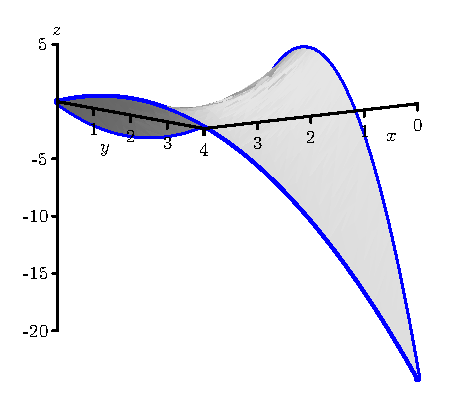
\includegraphics{figures/fig_10_7_activity_optim.eps}}
    \end{center}
    \caption{The domain of the function $f(x,y) = x^2-3y^2-4x+6y$ and
      its graph.}
    \label{F:10.7.Optimize_ex2}
  \end{figure}
  \ba
\item Find all of the critical points of $f$ in $R$.
	
\item Parameterize the horizontal leg of the triangular domain, and
  find the critical points of $f$ on that leg. 
\item Parameterize the vertical leg of the triangular
  domain, and find the critical points of $f$ on that leg. 
	
\item Parameterize the hypotenuse of the triangular domain, and find
  the critical points of $f$ on the hypotenuse. 
	
\item Find the absolute maximum and absolute minimum value of $f$ on
  $R$. 
	

	\ea
\end{activity}
\begin{smallhint}

\end{smallhint}
\begin{bighint}

\end{bighint}
\begin{activitySolution}
\ba
\item A direct calculation shows that $f_x = 2x-4$ and $f_y = -6y+6$. So $\nabla f = \vzero$ when $x=2$ and $y = 1$. This point is in the domain $D$ and is the only critical point of $f$ in $D$.

\item The base of the triangular domain can be parameterized by $x_1(t) = t$, $y_1(t) = 0$ with $t \in [0,4]$. Now
\[f_1(t) = f(x_1(t),y_1(t)) = f(t,0) = t^2-4t.\]
The critical points of $f_1$ are the roots of $f_1'(t)$. Now
\[f_1'(t) = 2t-4 = 0\]
when $t=2$. This give a critical point of $(2,0)$ on the base. We also need to consider the endpoints $t=0$ and $t=4$. When $t=0$ we have $(x,y) = (0,0)$ and when $t=4$ we have $(x,y) = (4,0)$. So there are three points at which $f_1$ can attain a maximum or minimum on the base of the triangular domain: $(2,0)$, $(0,0)$, and $(4,0)$.

\item The vertical leg of the triangular domain can be parameterized by $x_2(t) = 0$, $y_2(t) = t$ with $t \in [0,4]$. Now
\[f_2(t) = f(x_2(t),y_2(t)) = f(0,t) = -3t^2+6t.\]
The critical points of $f_2$ are the roots of $f_2'(t)$. Now
\[f_2'(t) = -6t+6 = 0\]
when $t=1$. This give a critical point of $(0,1)$ on the leg. We also need to consider the endpoints $t=0$ and $t=4$. When $t=0$ we have $(x,y) = (0,0)$ and when $t=4$ we have $(x,y) = (0,4)$. So there are three points at which $f_2$ can attain a maximum or minimum on the leg of the triangular domain: $(0,1)$, $(0,0)$, and $(0,4)$.

\item The hypotenuse of the triangular domain can be parameterized by $x_3(t) = t$, $y_3(t) = 4-t$ with $t \in [0,4]$. Now
\[f_3(t) = f(x_3(t),y_3(t)) = f(t,4-t) = t^2-3(4-t)^2-4t+6(4-t).\]
The critical points of $f_3$ are the roots of $f_3'(t)$. Now
\[f_3'(t) = 2t+6(4-t)-4-6 = 8t+14 = 0\]
when $t=-\frac{7}{4}$. This give a critical point of $\left(-\frac{7}{4},\frac{23}{4}\right)$ which is not in our domain. We also need to consider the endpoints $t=0$ and $t=4$. When $t=0$ we have $(x,y) = (0,4)$ and when $t=4$ we have $(x,y) = (4,0)$. So there are two points at which $f_3$ can attain a maximum or minimum on the hypotenuse of the triangular domain: $(0,4)$ and $(4,0)$.

\item We now only need to compare the values of $f$ at the critical points in the interior of $D$ and on the boundary of $D$. Now
\begin{itemize}
\item $f(2,1) = -1$,
\item $f(2,0) = -4$,
\item $f(0,0) = 0$,
\item $f(4,0) = 0$,
\item $f(0,1) = 3$,
\item $f(0,4) = -24$,
\end{itemize}
so the maximum value of $f$ on $D$ is 3, occurring at the point $(0,1)$ and the minimum value of $f$ on $D$ is $-24$, occurring at the point $(0,4)$.

\ea

\end{activitySolution}
\aftera
